\chapter{Análisis Experimental}
En esta sección se presenta la descripción de los escenarios , la plataforma de ejecución y el análisis experimental.

Este se divide en dos etapas, primero se realiza la configuración paramétrica para encontrar la mejor ejecución del algoritmo. Luego se realizan las pruebas donde se comparan los resultados entre los distintos escenarios.


\section{Desarrollo y Plataforma de ejecución }
Los algoritmos fueron desarrollados usando la biblioteca Malva que fue extendida en el código base para soportar la creación de nuevos hilos de ejecución para lograr el funcionamiento en paralelo.

Los escenarios fueron ejecutados en el cluster fing.

Cluster: Es un conjunto de computadoras independientes conectadas para que trabajen integradas como un solo sistema. De esta forma se consigue un alto rendimiento en la ejecución de tareas. 

Cluster Fing: Es una infraestructura de alto desempeño, que brinda soporte en la resolución de problemas complejos que demandan un gran poder de computo.

Descripcion del hardware: 
\begin{itemize}
	\item 9 servidores de cómputo
	\subitem Quad core Xeon E5430, 2x6 MB caché, 2.66GHz, 1.333 MHz FSB.
	\subitem 8 GB de memoria por nodo.
	\subitem Adaptador de red dual (2 puertos Gigabit Ethernet).
	\subitem  Arquitectura de 64 bits.
	\subitem Servidor de archivos: 2 discos de 1 TB, capacidad ampliable a 10 TB.
	\subitem Nodos de cómputo: discos de 80 GB.
	\item Switch de comunicaciones
	\subitem Dell Power Connect, 24 puertos Gigabit Ethernet.
	\item Switch KVM (16 puertos) y consola.
	\item UPS APC Smart RT 8000VA.
\end{itemize}

\section{Ajuste de parámetros de algoritmos}
Se busca la mejor configuración inicial de los parámetros realizando pruebas experimentales con diferentes combinaciones.  

\begin{itemize}
	\item Tiempo de simulación	
	\item Criterio de parada
	\item Tamaño de la población
	\item Probabilidad de mutación
	\item Probabilidad de cruzamiento
\end{itemize}

Para la realización de las pruebas se generan tres instancias con densidades de tráfico diferentes para realizar las pruebas de configuración. En este caso no se utilizan datos recabados de la realidad como  el trafico especifico de las calles y el recorrido de las lineas de omnibus. De esta forma el algoritmo queda genérico y no sesgado a un caso en particular.


\begin{itemize}
	\item Tráfico Bajo: 30 ómnibus y 500 vehículos	
	\item Tráfico Medio: 60 ómnibus y 1000 vehículos
	\item Tráfico Alto: 120 ómnibus y 2000 vehículos
\end{itemize}



En general se realizan entre 9 y 21 pruebas individuales en cada prueba para lograr mejor confiabilidad estadística usando los tres instancias de trafico generado.

En este proceso primero se define el tiempo de simulación y el criterio de parada, luego de establecidos se realizan las pruebas para todas las combinaciones de tasa de cruzamiento y mutación buscando los mejores valores para optimizar el algoritmo.

Al estar utilizando un cluster tenemos a nuestra disposición tanto la métrica del tiempo real que llevo la ejecución, así como también el tiempo secuencial es decir la suma del tiempo de procesamiento de todos los procesadores involucrados en la evaluación del algoritmo. 
A saber en las comparaciones del tiempo de ejecución se refiere al tiempo secuencial que es más confiable al no tener el sesgo dado por la cantidad de procesadores utilizados en la evaluación.
En general para las diversas pruebas se utilizaron entre 4 y 32 procesadores.



\subsection{Pesos de la función fitness}

Para las siguientes pruebas la función fitness (\ref{eq:funcion_fitness}) tendrá los pesos x = y = 1. Esto da pesos equitativos tanto a ómnibus como a otros vehículos por lo que no existe prioridad para uno u otro. Mas adelante se realizaran experimentos con otras variantes de los pesos.


\subsection{Tiempo de simulación}

Para tener un mejor control sobre los tiempos totales de ejecución, se busca encontrar un número fijo para el tiempo de la simulación de cada escenario que se ejecutará para cada solución.

Teniendo en cuenta que cada simulación de los escenarios representan el tráfico vehicular durante una hora real y que se validó que en cada escenario más de los 80 \% de los vehículos hayan dejado la simulación, es decir llegado a sus destinos.

Se establece un tiempo de simulación de 4000 steps (medida interna de tiempo del simulador SUMO equivalente a 66 minutos reales) que cumple con los criterios establecidos. 

\subsection{Criterio de Parada}
Se elige como criterio de parada el número de generación, esto permite estandarizar las pruebas para una mejor comparación.

Para determinar el número de generación donde parar el algoritmo se busca un compromiso entre un buen resultado y un tiempo de ejecución apropiado que no sea excesivo.

Para esto se decide que por un lado la ejecución del algoritmo deberá estar comprendida entre 1h y 24h y además comprobar experimentalmente que el valor de fitness no tiene una gran variación en las ultimas 100 generaciones.

Luego de la realización de las pruebas se elige el número de 500 generaciones como criterio de parada, como se ve en la siguiente gráfica representativa de las pruebas realizadas se aprecia como el valor de fitness no presenta grandes variaciones luego de la generación 400 ademas el tiempo de ejecución real esta dentro del margen pautado.




\begin{figure}[h]
\centering
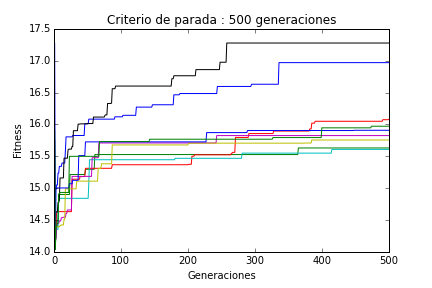
\includegraphics[width=0.7\linewidth]{Figures/criterio_parada}
\caption{Resumen representativo de ejecuciones del algoritmo para establecer el criterio de parada.}
\label{fig:criterio_parada}
\end{figure}



\subsection{Tamaño de la población}

Para la elección de la población se tendrán en cuenta 3 elementos. El valor de fitness encontrado, el tiempo de ejecución total y la plataforma de ejecución.

Dado que estamos ejecutando en el cluster y la máxima cantidad de procesadores que se pueden utilizar son 64 en un mismo nodo y teniendo en cuenta que la mejor distribución del trabajo es un elemento de población por procesador, se tiene que la máxima cantidad de población que estudiaremos sera 64.

Luego se eligen los valores 32 y 48 para completar el análisis teniendo en cuenta que no son lo suficientemente bajos como 8 u 16 y son valores con los que se obtiene una distribución más adecuada.

La siguiente tabla muestra los resultados obtenidos, como se aprecia no existen grandes diferencias en la elección de un número poblacional sobre otro. Por tanto se elige como número de población 32 teniendo en cuenta el tiempo de ejecución secuencial del algoritmo que como se aprecia es el menor. Se elige esta métrica por que aunque al ejecutar en paralelo el tiempo real que se puede obtener utilizando la máxima cantidad de procesadores para cada población son similares también se tiene en cuenta la disponibilidad y utilización de recursos que insume en el cluster fing. Por ejemplo obtener 64 procesadores para utilizar por un proceso en el cluster es algo que puede demorar varios días por la cantidad de otros procesos que también están funcionando en la plataforma y como se ve la ganancia que tenemos es mínima.

\begin{table}[h]
	\renewcommand{\arraystretch}{1.2}
	\caption{Comparación de fitness para distintas poblaciones}
	\label{table:parametro_poblacion}
	\centering
	\begin{tabular}{ccrrcr}
		\hline
		\multirow{2}{*}{\textbf{población}} & & 
		\multicolumn{2}{c}{\textbf{Fitness}} \\
		\cline{3-4}
		& & \multicolumn{1}{c}{mejor} 
		& \multicolumn{1}{c}{promedio} 
		& \multicolumn{1}{c}{tiempo de ejecución(m)} \\
		\hline
		32 & & \textbf{17.28} & 16.37$\pm$0.5 & 4853\\
		48 & & \textbf{16.19} & 15.84$\pm$0.3 & 6772\\
		64 & & \textbf{17.27} & 16.46$\pm$0.6 & 10184\\
		\hline
	\end{tabular}
\end{table}




\subsection{Probabilidad de mutación y cruzamiento}

Los valores elegidos fueron:

\begin{itemize}
	\item Probabilidad de cruzamiento (pc):  0.5, 0.8, 1
	\item Probabilidad de  mutación (pm):  0.01, 0.05, 0.1
\end{itemize}

Se realizan tres juegos de trafico diferente (bajo, medio y alto) y se realizan tres pruebas sobre cada uno, luego se ejecutan las nueve combinaciones de cruzamiento y mutación obteniendo el promedio del fitness para cada combinación con su desviación estándar.


 
 \begin{table}[h]
 	\renewcommand{\arraystretch}{1.2}
 	\caption{Combinaciones de probabilidad de cruzamiento(pc) y de mutación (pm)}
 	\label{table:parametro_mutacion_cruzamiento}
 	\centering
 	\begin{tabular}{p{1cm}p{1cm}p{3.5cm} }
 		\hline
 		$p_C$& 
 		$p_M$ & 
 		Fitness promedio  $\pm$ desviación estándar\\ 
 		\hline
 		0.5 & 0.01  &  16.09$\pm$0.30\\
 		0.5 & 0.05 &  15.60$\pm$0.17\\
 		0.5 & 0.1  &  16.16$\pm$0.42\\
 		0.8 & 0.01  &  16.04$\pm$0.55\\
 		0.8 & 0.05  &  15.85$\pm$0.32\\
 		0.8 & 0.1  &  16.08$\pm$0.34\\
 		1 & 0.01 &  16.08$\pm$0.45\\
 		1 & 0.05 &  15.82$\pm$0.34\\
 		1 & 0.1 &  16.04$\pm$0.25\\
 		\hline
 	\end{tabular}
 \end{table}
 
 
 

\begin{figure}[h]
	\centering
	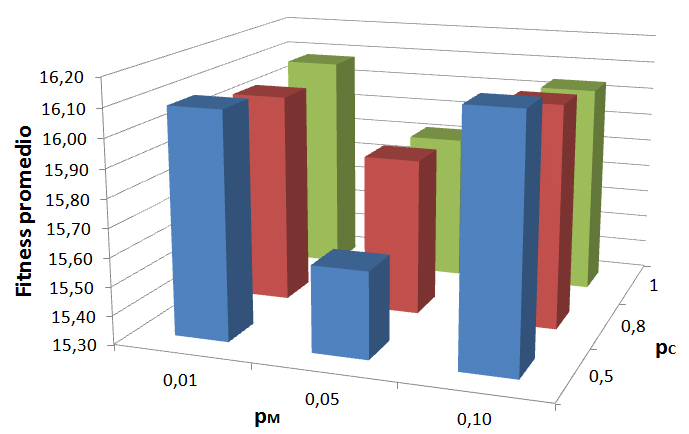
\includegraphics[width=0.7\linewidth]{Figures/grafica_mutacion_cruzamiento}
	\caption{Gráfica con combinaciones de probabilidad de cruzamiento(pc) y de mutación (pm)}
	\label{fig:grafica_mutacion_cruzamiento}
\end{figure}

Analizando la tabla y la gráfica se puede apreciar claramente que para una probabilidad de mutación de 0.05 se obtienen los peores resultados. Otro dato interesante es que no existe gran diferencia en el resto de las combinaciones.

Se comprueba que todas las muestras siguen la distribución normal  para poder aplicar el test de Student.

Siendo las hipótesis de la prueba ( u1 el promedio del  grupo 1 y u2 el del grupo 2) \newline
H0: u1  = u2  \newline
H1: u1 != u2 \newline

Si hacemos una comparación entre la combinación del mejor promedio (0.5-0.1) y del peor (0.5-0.05) con el test de Student obtenemos t(x) = 0.07 que nos indica que para un nivel de significancia de  0,1 la hipótesis nula es rechazada por lo tanto existe evidencia estadística para elegir la combinación con el mejor promedio (0.5-0.1) sobre la combinación con el peor promedio (0.5-0.05) para la ejecución del algoritmo.

Para comprobar si es la mejor opción  se toman las dos combinaciones con el mejor promedio (0.5-0.1) y (0.5-0.01) obteniendo en el test Student t(x) = 0.71 que nos indica que no existe una diferencia significativa entre ambas muestras por lo que elegir una sobre otra no implicaría grandes beneficios.

En tal sentido podríamos elegir cualquiera de las dos, en este caso se elige  la combinación (0.5-0.01) por su buen promedio y baja desviación estándar.



\section{Descripción de escenarios}
En todos los escenarios se utiliza los datos del tráfico vehicular, configuración de semáforos y frecuencia de los ómnibus obtenidos. 

\subsection{Caso base}
Esto representa la situación actual en términos de tráfico, red vial y sincronización de semáforos del corredor Garzón. 

Se valida su correctitud comparando los tiempos obtenidos en la simulación con tiempos obtenidos in-situ de los recorridos de ida y vuelta para los vehículos. Y utilizando las frecuencias de acceso publico en el caso de los ómnibus.

Se realizo un estudio sobre datos proporcionados por la IMM que contenían el posicionamiento de los ómnibus, velocidad instantánea y datos de la linea durante todo el día para una semana en particular. De esta forma se constato que para de las lineas de ómnibus que pasan por Garzón la  velocidad promedio de los ómnibus es de 14.5km/h.

Esto permitió calibrar el caso base modificando aspectos de la simulación relacionados con los ómnibus haciéndolo mas preciso.

Sobre este escenario se realizaran tres instancias de trafico : bajo, medio y alto.
El caso medio representa los datos obtenidos, el bajo es aplicando una disminución del 50\% de vehículos y disminuyendo el tiempo de espera en las paradas de ómnibus teniendo en cuenta que en este caso existirá menos personas bajando y subiendo del ómnibus. Las frecuencias de ómnibus se mantienen iguales ya que no son alteradas en la realidad.
El caso de alto trafico se realiza un aumento del 50 \% de los vehículos y se aumenta el tiempo de espera en la parada de los ómnibus.

El aumento y disminución del 50\% se obtuvo al analizar datos proporcionados por la IMM de la zona de Garzón de años anteriores. \newline

Alto Trafico: Cerca de 2800 vehiculos en la simulacion y 70 omnibuses. \newline
Trafico Medio: Cerca de 2000 vehiculos y 70 omnbibueses \newline
Trafico Bajo: Cerca de 1000 vehiculos y 70 omnibuses
 

\subsection{Escenario Evolutivo }
En este caso se ejecuta el algoritmo evolutivo sobre el caso base para obtener una nueva sincronización de semáforos optimizada que repercutirá en la calidad del tráfico.

En este caso se realizan 21 ejecuciones independientes sobre cada instancia de trafico.


\subsection{Escenario Alternativo}

Para mostrar la utilidad que tienen las simulaciones sobre un escenario real, se realiza solo a modo de ejemplo un escenario alternativo. Una de las ventajas principales es que no requiere gran inversión monetaria, de tiempo y que no afecta la situación actual de la realidad, por lo que se pueden generar distintas pruebas para encontrar aquellas que logren un beneficio.

Analizando aquellos puntos que se entienden podrían atentar contra el buen funcionamiento del Corredor, se agregan algunas modificaciones al escenario base para intentar mejorarlo. 

El objetivo no es demostrar que esta sera la mejor alternativa sino dar una de las muchas alternativas que se pueden generar y probar con la simulación si se logran mejoras. Ya que pueden existir limitaciones o reglas que no estamos tomando en cuenta y que deben cumplirse en la realidad.

-Limitar cruces a la izquierda

-Eliminar paradas

-Agregar calles paralelas a Garzon

-


\section{Resultados}
Presentaremos los resultados obtenidos  utilizando los parámetros óptimos  para el escenario base, el escenario alternativo, y la prueba en el cluster.

\subsection{Resultado simulación caso base}

En la tabla se pueden ver las métricas obtenidas para los diferentes instancias de trafico simulado.
 
 \begin{table}[h]
 	\renewcommand{\arraystretch}{1.2}
 	\caption{Resultados caso base, velocidad promedio bus (vpb) y velocidad promedio vehículos(vpv) }
 	\label{table:resultado_caso_base}
 	\centering
 	\begin{tabular}{p{2.5cm}p{2.5cm}p{2.5cm}p{2cm} }
 		\hline
 		&
 		$vbp(km/h)$& 
 		$vvp(km/h)$ & 
 		Fitness \\ 
 		\hline
 		Trafico Bajo & 15.89  & 32.45& 13.42\\
 		Trafico Medio & 14.59  & 28.81& 12.05\\
 		Trafico Alto & 14.31  & 26.36& 11.30\\

 		\hline
 	\end{tabular}
 \end{table}


\subsection{Resultado Escenario Evolutivo}


\begin{table}[h]
	\renewcommand{\arraystretch}{1.2}
	\caption{Resultados Algoritmo, velocidad promedio bus (vpb) y velocidad promedio vehículos(vpv) }
	\label{table:resultado_caso_algoritmo}
	\centering
	\begin{tabular}{p{2.5cm}p{2.5cm}p{2.5cm}p{2cm}p{2cm} }
		\hline
		&
		$vbp(km/h)$& 
		$vvp(km/h)$ & 
		Fitness &
		Mejora(\%)
		\\ 
		\hline
		Trafico Bajo & 17.92  & 34.30& 14.50$\pm$0.14 & 8\\
		Trafico Medio & 16.95  & 33.29& 13.95$\pm$0.15 & 15.70\\
		Trafico Alto & 16.51  & 32.90& 13.72$\pm$0.17 & 21.40\\
		
		\hline
	\end{tabular}
\end{table}

Se realizaron 21 ejecuciones independientes para cada tipo de trafico comprobando que siguieran una distribución normal.

Por tanto se puede aplicar el criterio de significancia estadística para validar los resultados, que dice que el
algoritmo A es mejor que el algoritmo B si los resultados de A y B cumplen:


\begin{equation}
\label{eq:funcion_significancia}
\left |f_{avg}(A) - f_{avg}(B)  \right | > max(std(f_A),std(f_B))
\end{equation}

En este caso A representa el algoritmo y B el caso base. Esto indica que la diferencia del resultado promedio del caso base restado al resultado del caso base debe ser mayor a la máxima desviación.
Esto se cumple para todos los casos, por lo que podemos afirmar que existe evidencia estadística para decir que los resultados del algoritmo son mejores al del caso base.


Esto significa que un viaje en ómnibus del principio al fin del corredor (6.5km) duraba 27min en el caso base y luego del algoritmo se mejora hasta 23.5min en una situación de trafico alto. En el caso de un viaje en auto la duración era de 14.8min y luego del algoritmo 11.8min.

Al analizar la tabla se ve que los resultados del algoritmo para trafico alto son aun mejores que el trafico bajo en el caso base. 





\subsection{Resultado Escenario Alternativo}

\subsection{Comparación Secuencial vs  Paralelo}

El speedup se define como T1/Tp
T1 es el tiempo de ejecucion en un procesador
Tp es el tiempo de ejecucion en p procesdores.


Vamos a comprobar la utilidad de tener un algoritmo paralelo comparando el tiempo de ejecucion en diferentes número de procesadores

La escabilidad de un algoritmo define su capacidad para aumentar su rendimiento a medida que se agregan más procesadores.

En este caso comparamos el algoritmo ejecutado en 1, 8, 16, 32 procesadores.



\begin{table}[h]
	\renewcommand{\arraystretch}{1.2}
	\caption{Analisis de speedup }
	\label{table:analisis_speedup}
	\centering
	\begin{tabular}{p{2.5cm}p{2.5cm}p{2.5cm} }
		\hline

		Procesadores& 
		Tiempo(m) & 
		Speedup 
		\\ 
		\hline
		1  & 11399 & 1\\
		4  & 1936 & 5.8 \\
		8  & 1491 & 7.6 \\
		16  & 803 & 14.1 \\
		\hline
	\end{tabular}
\end{table}
GRAFICA DE ESCABILIDAD

El comando "time" ejecutado sobre nuestro algoritmo nos brinda el tiempo real de ejecución, así como el tiempo total sumado de todos los procesadores. Por tanto podemos calcular el tiempo del algoritmo secuencial.

En el caso de 8 procesadores, al tener una población de 32 se distribuirán 4 individuos por procesador.

Por tanto cuando tenemos 32 es donde se logra la mejor distribución al no existir "overhead" en la creación y terminación de los hilos.


\subsection{Variación de la función de fitness}

La función fitness (\ref{eq:funcion_fitness}) utilizada para las pruebas tenia pesos x = y = 1 lo que representaba que se le daba un balance equitativo a ómnibus y vehículos.

Por un cruce de Garzón pasan cada hora:
70 ómnibus , si aproximamos con 23 personas= 1610 personas por hora
800 autos, si aproximamos  2 personas por vehículo nos da 1600 personas por hora.
Una cantidad similar  pasan por el cruce en ambos medios de transporte por lo que no existe una tendencia a favor de una sobre la otra, se podría aproximar que 50\% eligen el ómnibus y 50\% el auto.



Estos pesos pueden ser cambiados en función de lo que se necesite por lo que vamos a realizar pruebas con dos funciones de fitness diferentes sobre el escenario con trafico medio y comparar los valores de velocidades medias para cada tipo de vehículo.


\subsubsection{Prioridad ómnibus}
El primer caso se le dará mas prioridad a los ómnibus, esto se sostiene en el hecho que uno de los objetivos buscados por la IMM  es que se utilice mas el transporte colectivo (ref??). Con la premisa que al mejorar la duración del viaje en ómnibus relativo al del auto por el corredor las personas que utilizan auto para sus viajes opten por el transporte colectivo.

Por tanto vamos a experimentar con una nueva función fitness con un peso de 70\% para los ómnibus y 30\% al resto de los vehículos.

(TABLAS Y COMPARACIÓN)

\subsubsection{Prioridad otros vehículos}

En este caso, le damos 70\% del peso a los vehiculos y 30\% a los omnibus.

(RESULTADOS?)

Se podrian seguir variando los pesos hasta lograr una misma velocidad para omnibus y otrosvehiculos??


\section{Resumen}

